\chapter{Entorno virtual}
Uno de los principales objetivos de este trabajo es realizar pruebas funcionales y de escala sobre la arquitectura del prototipo. Es de interés generar distintas realidades, y así detectar puntos de falla o variables clave en la performance de la arquitectura. Para esto se puede utilizar dos parámetros: topología y servicios. Es importante poder aplicar topologias complejas y relativamente grandes a la arquitectura, así como grandes cantidades de servicios, y de esta forma encontrar posibles problemas con la arquitectura, y su respectiva solución. Dado que no es realista hacer este tipo de pruebas con un prototipo físico, por temas económicos y prácticos, se observa la necesidad de un entorno virtual capaz de simular las características del prototipo. En este capítulo se estudian los requerimientos que debe cumplir este entorno, las herramientas estudiadas para lograrlo, y los detalles de diseño e implementación de la solución construida.

\section{Requerimientos del entorno virtual}
Los requerimientos de este entorno se pueden dividir en dos grupos. En primer lugar, la idea es que el entorno virtual se comporte de una forma lo más fiel posible al prototipo físico. Esto no quiere decir que deba usar las mismas herramientas, pero es deseable que así sea. En segundo lugar, hay que considerar los requerimientos inherentes de un entorno de simulación como el que se pretende. El primer grupo se detalla a continuación.

\begin{itemize}
	\item Se debe poder simular múltiples RAUSwitch virtuales, y los mismos deben tener las mismas capacidades funcionales que sus pares físicos. A partir de esto, se desprenden los siguientes sub-requerimientos.
	\begin{itemize}
		\item Deben poder ejecutar el protocolo de enrutamiento OSPF. Es deseable que lo hagan mediante la suite de ruteo Quagga.
		\item Deben soportar el protocolo OpenFlow 1.3. Esto se debe a que la aplicación que implementa VPNs depende de que los switches tengan soporte para MPLS, y OpenFlow ofrece esta funcionalidad a partir de la versión 1.3 (???). Es muy deseable que lo hagan mediante OpenVSwitch, ya que es lo que utilizan los RAUSwitch físicos.
	\end{itemize}
	\item Se debe poder simular múltiples hosts, ya que son los agentes que se conectan a la red y se envían tráfico entre sí, para corroborar que los flujos de datos son correctos.
	\item La aplicación RAUFlow debe ejecutarse y comunicarse correctamente con los RAUSwitch. Esto implica que el controlador Ryu debe ser soportado por el entorno.
\end{itemize}

Cabe remarcar que los módulos SNMP y LSDB Sync quedan por fuera de los requerimientos principales, por ser no esenciales. \\

El segundo grupo de requerimientos es más genérico, ya que son los que surgen para casi cualquier entorno de simulación de redes.

\begin{itemize} 
	\item Facilidad de configuración. Es importante que el entorno pueda generar distintas topologias y escenarios sin demasiado esfuerzo de configuración.
	\item Escalabilidad. Dado que uno de los objetivos es realizar pruebas de escala, el entorno debería ofrecer buena escalabilidad en la cantidad de nodos que puede simular. Esto se traduce a que una computadora promedio de uso personal pueda levantar algunas decenas de nodos virtuales como mínimo.
\end{itemize}

\section{¿Por qué Mininet?}


\section{Diseño e implementación del entorno}
El entorno está construido alrededor de Mininet, y se podría pensar como una extensión de la misma. \textit{Out of the box}, Mininet ya cumple la mayoría de los requerimientos estudiados anteriormente. Está diseñada para ser escalable, ya que usa containers reducidos, tiene soporte para OpenFlow 1.3 mediante OpenVSwitch, y gracias a su API en Python es muy fácil de configurar. El aspecto en el que falla es en el soporte para Quagga. Dado que Mininet es una herramienta de prototipado para SDN puro, no está pensado para un esquema híbrido como el que se propone. Los switches compatibles con OpenVSwitch que ofrece no pueden tener su propio network namespace, por lo tanto, no pueden tener su propia tabla de ruteo ni interfaces de red aisladas, así que no es posible que utilicen Quagga.

Por otro lado, los hosts de Mininet sí tienen su propio network namespace, y gracias a su capacidad de tener sus propios procesos y directorios, podemos ejecutar una instancia de Quagga y OpenVSwitch para cada host. De esta forma es posible crear un router como el requerido por la arquitectura. Esta extensión de las funcionalidades de los hosts es posible ya que Mininet está programado con orientación a objetos y permite al usuario crear subclases propias de las clases que vienen por defecto. En la figura \ref{fig:clases_entorno} se puede ver la estructura de clases del entorno construido. En las siguientes secciones se procederá a estudiar cada una de ellas.

\begin{figure}[t]
	\caption{Diagrama de clases del entorno.}
	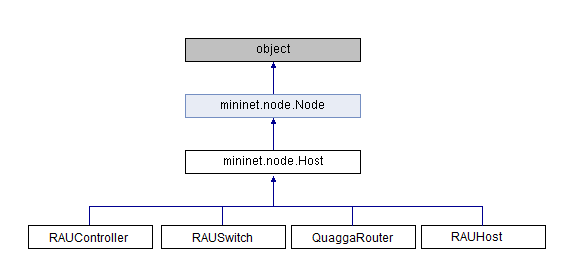
\includegraphics[scale=0.65]{Entorno/clases_entorno}
	\centering
	\label{fig:clases_entorno}
\end{figure}

\subsection{RAUController}
En el uso típico de Mininet, la comunicación entre el controlador y el switch se da a través de la interfaz de loopback. Esto es así porque los switches no tienen su propio namespace. Para lograr dicha comunicación, no hace falta un objeto en Mininet que represente el controlador, ya que ejecutar la aplicación en el sistema operativo base ya habilita al switch a comunicarse con ella a través de la interfaz de loopback. Esta situación cambia en este diseño, porque los switches pasan a tener su propio network namespace. Esto lleva a la necesidad de crear un host virtual, que ejecute la aplicación de RAUFlow y se comunique con los switches a través de enlaces virtuales. Para satisfacer esta necesidad se usa la clase RAUController.

\subsection{RAUSwitch}
La clase RAUSwitch es el núcleo del entorno de simulación. Es un Host extendido de tal forma para que, gracias a la funcionalidad de directorios privados, ejecute su propia instancia de Quagga y OpenVSwitch. Cada RAUSwitch tiene los siguientes directorios privados: /var/log/, /var/log/quagga, /var/run, /var/run/quagga, /var/run/openvswitch. Cada RAUSwitch también usa un directorio bajo /tmp, para almacenar sus archivos de configuración.\\ \\

OpenVSwitch básicamente consiste de 2 demonios (ovs-vswitchd y ovsdb-server) que ejecutan en el user-space, y un módulo en el kernel que actúa como cache para los flujos recientes. Utiliza el protocolo 'netlink' para comunicar el user-space con el módulo en el kernel. Poder tomar decisiones sobre los paquetes a nivel del kernel, sin tener que pasar por el user-space, explica en gran medida el buen nivel de performance que ofrece OpenVSwitch. Sin embargo, tener múltiples módulos de kernel ejecutando en el mismo sistema operativo puede crear comportamientos impredecibles e incorrectos, ya que no está previsto para trabajar de esa forma.\\
Afortunadamente, OpenVSwitch puede ejecutarse completamente en modo user-space, es decir, sin soporte del módulo del kernel. Esto implica que podemos ejecutar tantas instancias de OpenVSwitch como queramos, pero la performance va a ser significativamente peor. Esto no es una desventaja muy seria, ya que el objetivo del entorno no es ser performante al procesar paquetes. Cabe aclarar que en este modo OpenVSwitch continúa haciendo cacheo de flujos, pero ahora lo hace en el user-space.

\begin{figure}[t]
	\caption{Arquitectura de OpenVSwitch.}
	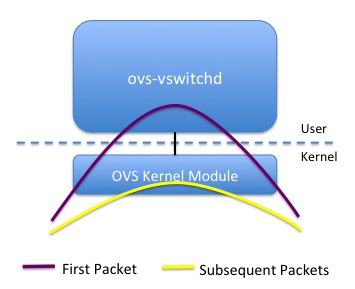
\includegraphics[scale=0.65]{Entorno/ovs_dataplane}
	\centering
	\label{fig:ovs_dataplane}
\end{figure}

\subsection{QuaggaRouter}
Es una clase similar al RAUSwitch pero sin OpenVSwitch, es decir, sólo usa Quagga. Apunta a representar el router CE que utilizaría una subred para conectarse a la red. Está conectado a un RAUSwitch de borde.

\subsection{RAUHost}
Representa a los hosts que serán clientes de la red. Con este propósito, se podría utilizar directamente la clase Host de Mininet, pero se construye esta clase auxiliar para evitar determinadas configuraciones manuales, como por ejemplo, el \textit{default gateway}.


\section{Modo de uso del entorno}
En Mininet estándar, las topologias se crean mediante la API en Python. Se crea un objeto de tipo Topology, se le agregan los nodos que se desee, y se establecen los enlaces virtuales entre esos nodos. Como el entorno es en esencia una extensión de Mininet, hereda su facilidad de uso. La única diferencia radica en que las entidades de este entorno requieren parámetros adicionales para su creación, que serán detallados en el Anexo.
